\documentclass[conference,11pt]{article}
\usepackage[top=1in, bottom=1in, left=1in, right=1in]{geometry}
\usepackage{amsmath,amsthm,amssymb,algorithm,algorithmic}
\usepackage{graphicx}
\title{\textbf{Machine Learning with Soccer Game Prediction}}
\author{Yi Ou \and Jiani Lin}
\begin{document}
\maketitle

\section{Introduction}
\subsection{The problem}
In Europe and South America, soccer is one of the most popular sport. People find interest in soccer game for various reasons and at different levels. One of them is that soccer is an excellent game for different forms of betting. The outcome of a soccer match depends on many factors, except for the factors that can be easily measured by data, there exists some factors like the mood of players and the body condition of players, and some situation like the effect of injured players and various psychological effects. 
\subsection{Why it is interesting}
The charm of the football games, not only appears on its dedication to the extremely exciting competitions, but also has its own unpredictability, it seems random that affected by many factors, such as the mental state of the players, the weather, or the field of competition . Above all, many companies may use sports lotteries to win the benefits, some other men also bet on the output of a competition which they think is very exciting. However, all these things rely on the results of the English Premier League, so how can we maximize the benefits? The soccer competition predicting now appears particularly important. 

\section{Mainly work}
\subsection{Data set}
Our data set mainly from the website http://www.football-data.co.uk/data.php, which is a professional football data website had datasets including fulltime and halftime results for up to 22 European league divisions from 19
seasons back to 1993/94.\\ 
In detail, the website have lots of match statistics may be useful for us,  like shots, shots
on goal, corners, fouls, offsides, yellow card, red card and referees. Betting odds for each match were also
available from multiple betting websites.

\subsection{Feature Selection}
Based on the experience as a soccer fan, and reference of others' researches, we extract the features as follow:
\begin{enumerate}
\item \textbf{FIT-MATCH-K}:
The previous K game result of each team. $result = \{H,D,A\}$, which labeled as $result = \{3,1,0\}$. The result presents the points a team gain from the latest K games, which can indicate the state of performance of this team to some degree, it's a significant feature used to predict the game results.
\item \textbf{HISTORY-K}:
The previous K season of game result between the home team and away team. $result = \{H,D,A\}$, which labeled as $result = \{3,1,0\}$. This feature show that the history game performance when they play against each other, which can indicate the state of performance of both team, especially, there exists several teams that always win when play against certain teams.
\item \textbf{AVG-SHOTS-K}:
The average number of shots made in the  previous K game of each team. It can reflex the lately attack performance of the teams.
\item \textbf{AVG-SOT-K}:
The average number of shots on target made in the previous K game of each team. It's also a feature can reflex the lately attack performance of the teams.
\item \textbf{AVG-CORNER-K}:
The average number of corners made in the previous K game of each team. It's also a feature can reflex the lately attack performance of the teams.
\item \textbf{AVG-FOUL-K}:
The average number of foul made in the previous K game of each team. It can show that the lately defense performance of the teams.
\end{enumerate}

\subsection{Feature Extraction}
It's a little bit trick that when we use the MATCH-K feature, it's a list contains K game results of both teams. For example, if $K = 6$, $Result_{home team} = \{3,0,1,0,1,3\}$, $Result_{away team} = \{1,1,1,3,1,3\}$.And we conduct the first algorithm as follow :\\
\begin{equation}
MATCH_K = \sum_{i=1}^{K}Result_{home team, i}/K - \sum_{i=1}^{K}Result_{away team, i}/K
\end{equation}
The algorithm just simply use the average of K games of home team to minus the average of K games of away team, and we can find that the algorithm put same weight on each games, which is not reasonable enough. Denote the weight of each game as $w_i$, In common sense, $w_i$ should be larger than $w_j$ if $i > j$, but we don't know the exactly weight of each game, so we decide to combine the previous K game of both teams and  learn the weight by linear fitting using the game of 2014-2015 season and 2015-2016 season.

\begin{center}
\begin{tabular}{|cccccccccccc|}
      \hline
             $w_1$ & $w_2$  & $w_3$ & $w_4$ & $w_5$ & $w_6$ &$w_7$ &$w_8$ &$w_9$ &$w_{10}$&$w_{11}$&$w_{12}$\\
      \hline
            -0.085  & -0.015 & 0.020 & 0.074 & 0.168 & 0.121& -0.016 &-0.139 &0.029 & -0.148 & -0.123 & -0.070\\
      \hline
\end{tabular}\\
\ \\
Table 1. Weight of MATCH-K
\end{center}
And use $y=w^Tx$ as the MATCH-K feature. 

\subsection{Training Set and Test Set}
Since the recent results can show the status of a team, and we induced the feature of the results of latest six game, we need to separate training set and test set carefully such that for each date the recent information  can be used in learning and the training set would not matriculate the test set. We use algorithm 1, where we add the an example into the training  set, only after getting the accuracy of perdition in this sample.
\begin{algorithm}
\caption{Select training set and test set}
\begin{algorithmic}
\STATE{Trainset=\{ all games in season 13 and 14\}}
\STATE{Data={games in season 15}}
\STATE{n=length(Date)}
\STATE{sort games in Date by time, the latest game is in the last}
\FOR{ n =1 \textbf{to} n}
\STATE{train(Trainset)}
\STATE{test(Data(i))}
\STATE{Trainset.append(Data(i))}
\STATE{i=i+1}
\ENDFOR
\end{algorithmic}
\end{algorithm}

\subsection{Gambling Odds}
As the gambling company will provide betting odds before the match, we expect to take betting odds as a standard line to test the accuracy of our method. We have tried to predict the result only by betting odds from different gambling company, using logistic regression:
\begin{equation}
h_\theta(z)=\frac{1}{1+e^-z} \qquad \textrm{where} \quad z=\theta^Tx
\end{equation}
if $h(\theta) \geq 0.5$, predict true, else predict false. We can find optimal theta by minimize the cost function:
\begin{equation}
\textrm{J}(h_\theta, y)=-y\log(h_\theta(x))-(1-y)\log(1-h_\theta(x))
\end{equation}
where, y means the label of data. We train this algorithm on season 2014, and test season 2015. The accuracy of correctly predicting if the home team can win is $67.63\%$. Then by using multi-class classification, we got the accuracy of predicting result (home win, away win and draw) with $47.37\%$.

\section{Ideas From Class}

\subsection{Multi-class Classification}
Soccer result prediction is a multi-class classfication problem, the result we should predict from the set $\{H,D,A\}$, $H$ means the home team win the game, $D$ represents the draw condition, and $A$ means the home team lose. Specifically, we use one-vs-all algorithm to combine our linear classifiers.
\subsection{Logistic Regression}
We choose Logistic Regression as one of our linear classifiers because we think our features are independent and it's suitable to try Logistic Regression learning our problem. Logistic Regression is an outstanding linear classifier measures the relationship between the categorical dependent variable and one or more independent variables by estimating probabilities using a logistic function, which is the cumulative logistic distribution. 
\subsection{Support Vector Machine}
SVM is a strong classifier which not only can do linear classification, but also can efficiently perform a non-linear classification using what is called the kernel trick, in our paper, we try linear kernel and Gauss kernel as our kernel, and compare their efficiency when predicting the game results.

\section{What We learned}
During the project, we learned lots of things from datasets collection to comparing different result. Data collection is the preparation for the machine learning project, when you decide to learning a problem you interested, think about if you can collect enough efficient data, if you don't have enough data, there is no way you can train a efficient model or extract enough features for learning, which means you can't get a decent result. Then is feature selection and extraction, firstly you should read enough papers to have a good notion about what features may effect the result of your problem, then try to extract or transform your data to a useful feature. About learning, large training set doesn't always the good training set, like our problem, you can't use too many and too old data, because the regular pattern may be change sharply. For the most of the problem, you don't know the hypothesis space, in that situation, you should try enough different method and compare the results, then do some analysis about the results.

\section{Result}
We implemented and tuned 4 models, whose accuracy are illustrated in Figure 1.

\begin{center}
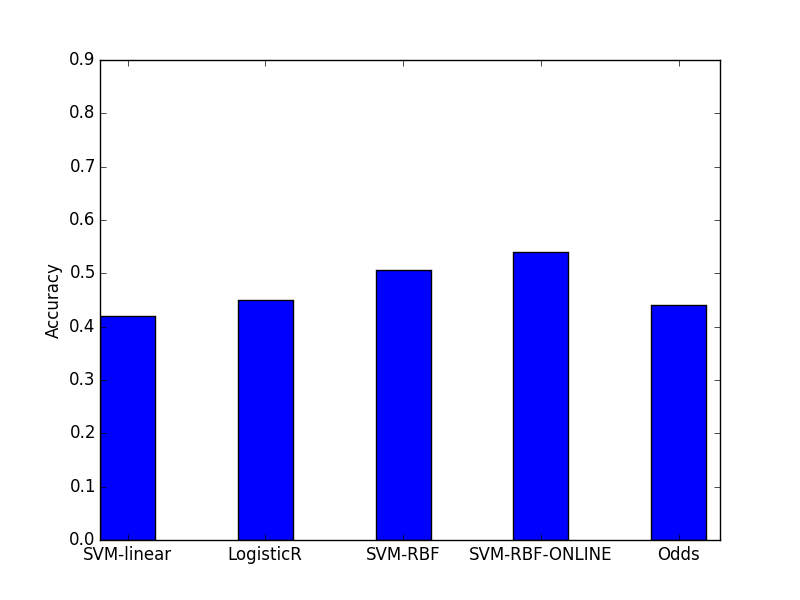
\includegraphics[scale = 0.5]{figure_1.png}\\
Figure 1. Accuracy of 4 models compare to odds
\end{center}
\ \\
And the accuracy respect to win, draw and lose are illustrated in Figure 2.

\begin{center}
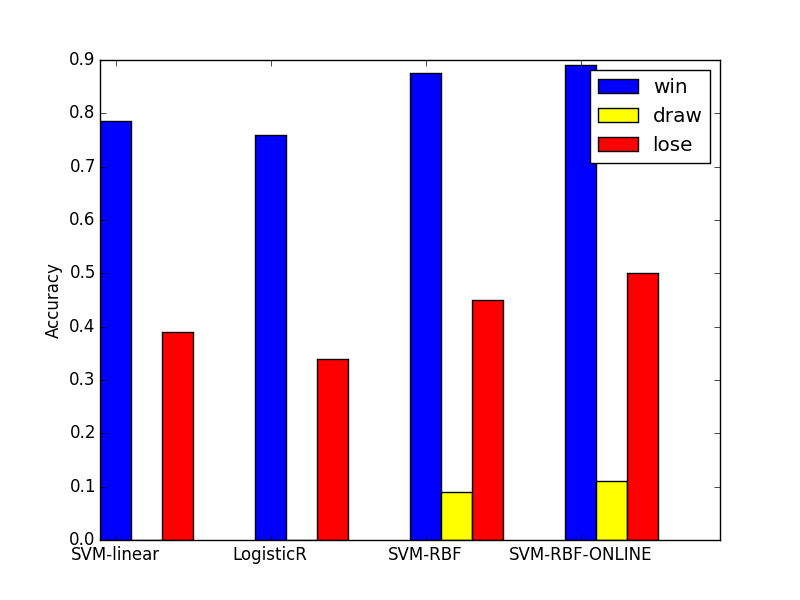
\includegraphics[scale = 0.5]{figure_2.png}\\
Figure 2. Accuracy of 4 models respect to win, draw, lose(away team win)
\end{center}
\ \\
\begin{center}

\begin{tabular}{|c|ccc|}
      \hline
      SVM-RBF-ONLINE       &Actual win & Actual draw  & Actual away \\
      \hline
      Predict win     & 50  & 23 & 24  \\
      Predict draw     & 2  & 5 &1\\
      Predict away     & 4 & 15 &26\\
      \hline
    \end{tabular}\\
    \ \\
    {\small Table.2 SVM-RBF-ONLINE Result Detail}
\end{center}
\ \\
The baseline of English Premier League is 37\%(home team win), 28\%(draw) and 35\%(away team win), our best result which achieved by SVM-RBF-ONLINE is 54\%, is 17\% better than the baseline. From Table.2 we can see that our best model SVM-RBF-ONLINE do an excellent job when the home team win with near 90\% accuracy, and around 50\% accuracy when home team lose. Unfortunately, we can't predict the result of draw, may be due to the high randomness of data when two teams draw.

\section{Perspective}
\subsection{More Feature}
\begin{enumerate}
\item{external factors}\\
Some external factors may be considered, like referee and the weather in that day. We will looking for the features in this category carefully to find some features affect the game indeed.
\item{Distance and Schedule}\\
A long travel sometimes will effect the performance of a team, and the schedule can also make an impact on the result, due to the players may fell tired during the tight period.
\item{others}\\
There are some factors which may affect the result significantly, such as illness of the players. We will identify more attributes in this type.
\end{enumerate}
%\end{enumerate}
\subsection{Try More Classifier}
\begin{enumerate}
\item if we have more time, we like to try more methods like Random Forest, Neutral Network and some heuristic algorithms.
\end{enumerate}

\subsection{Try other methods}
\begin{enumerate}
\item if we have more time, we like to try more methods like Markov random model, or some Time series analysis method. Furthermore, we may try to predict the game from other respect, like predicting uncommon game result, predicting game result based on player scores. 
\end{enumerate}

\subsection{Conduct a method to win money using our classifier}
\begin{enumerate}
\item Conducting a method based on the odds and our classifier to make money.
\end{enumerate}





\end{document}
